\documentclass[aspectratio=169]{beamer}

\usetheme{Madrid}
\usecolortheme{default}
\setbeamertemplate{footline}{%
  \leavevmode%
  \hbox{%
    \begin{beamercolorbox}[wd=.75\paperwidth,ht=2.5ex,dp=1ex,leftskip=1em]{author in head/foot}%
      Team 3 -- BG Bank RPC Project
    \end{beamercolorbox}%
    \begin{beamercolorbox}[wd=.25\paperwidth,ht=2.5ex,dp=1ex,center]{date in head/foot}%
      \insertframenumber{} / \inserttotalframenumber
    \end{beamercolorbox}%
  }%
}

\usepackage{graphicx}
\usepackage{booktabs}
\usepackage{array}

\graphicspath{{./}{ResultImage/}{Logo/}}

\title{BG Bank RPC Project}
\subtitle{Secure Banking Web Application}
\author{Team 3}
\institute{Institute of Technology of Cambodia\\Department of Applied Mathematics and Statistics}
\date{Introduction to Parallel and Distributed Systems\\I4-AMS-DAS-A (2025--2026)}

\begin{document}

\begin{frame}
    \titlepage
\end{frame}

\begin{frame}{Project Overview}
    \begin{itemize}
        \item BG Bank is a secure banking web application built with Flask and XML-RPC.
        \item The system separates the web interface, authentication service, banking service, and database.
        \item Users can register, log in, view a dashboard, deposit, withdraw, transfer, view history, and update profile information.
        \item The project demonstrates distributed service communication using Remote Procedure Call.
    \end{itemize}
\end{frame}

\begin{frame}{Project Objectives}
    \begin{itemize}
        \item Build a complete banking web application for customer account operations.
        \item Use XML-RPC for communication between the web app and backend services.
        \item Protect user sessions with encrypted login tickets.
        \item Require an action password for sensitive transactions.
        \item Store users, profiles, accounts, transactions, and audit logs in SQLite.
    \end{itemize}
\end{frame}

\begin{frame}{System Architecture}
    \centering
    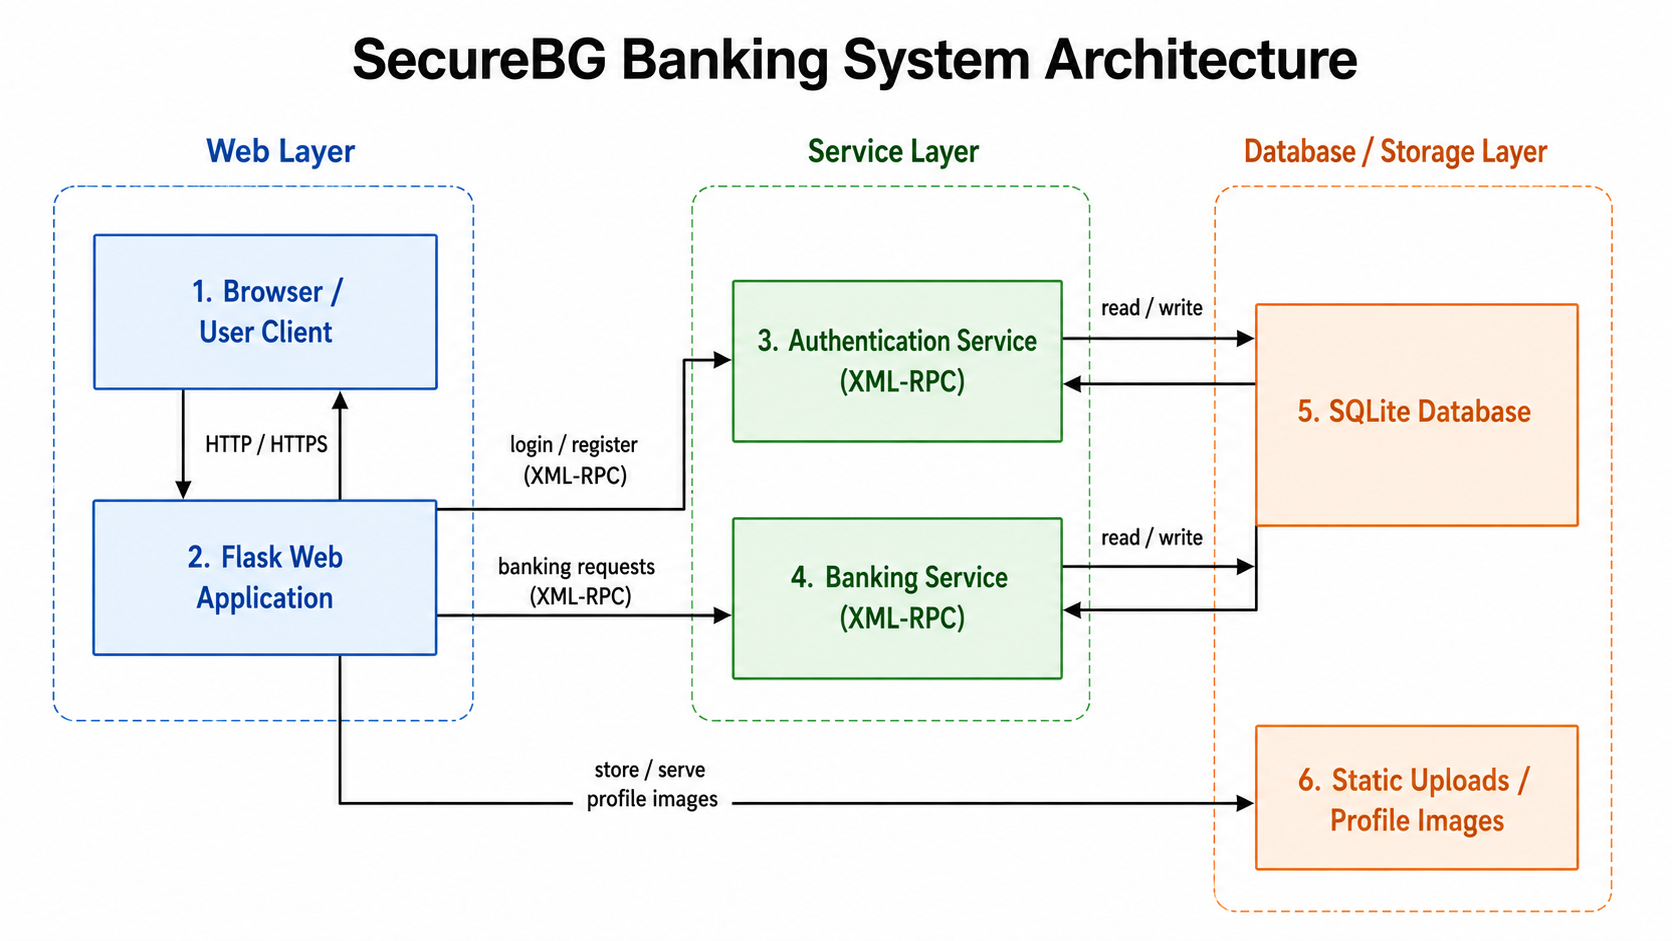
\includegraphics[width=0.92\textwidth,height=0.72\textheight,keepaspectratio]{System-Architecture-Diagram-GPT.png}
\end{frame}

\begin{frame}{Main Components}
    \begin{tabular}{p{0.28\textwidth} p{0.62\textwidth}}
        \toprule
        \textbf{Component} & \textbf{Responsibility} \\
        \midrule
        Browser & Displays pages and sends user requests to Flask. \\
        Flask Web App & Handles routes, forms, sessions, templates, and RPC calls. \\
        Authentication Service & Handles registration, login, password hashing, and ticket issuing. \\
        Banking Service & Handles balance, deposit, withdraw, transfer, history, dashboard, and profile operations. \\
        SQLite Database & Stores users, accounts, profiles, transactions, and audit logs. \\
        \bottomrule
    \end{tabular}
\end{frame}

\begin{frame}{RPC Service Design}
    \begin{columns}
        \begin{column}{0.48\textwidth}
            \textbf{Authentication RPC}
            \begin{itemize}
                \item \texttt{register\_user()}
                \item \texttt{login()}
                \item Issues encrypted login tickets
            \end{itemize}
        \end{column}
        \begin{column}{0.48\textwidth}
            \textbf{Banking RPC}
            \begin{itemize}
                \item \texttt{deposit()}
                \item \texttt{withdraw()}
                \item \texttt{transfer()}
                \item \texttt{view\_transaction\_history()}
                \item \texttt{get\_dashboard\_summary()}
            \end{itemize}
        \end{column}
    \end{columns}
\end{frame}

\begin{frame}{Transfer Workflow}
    \centering
    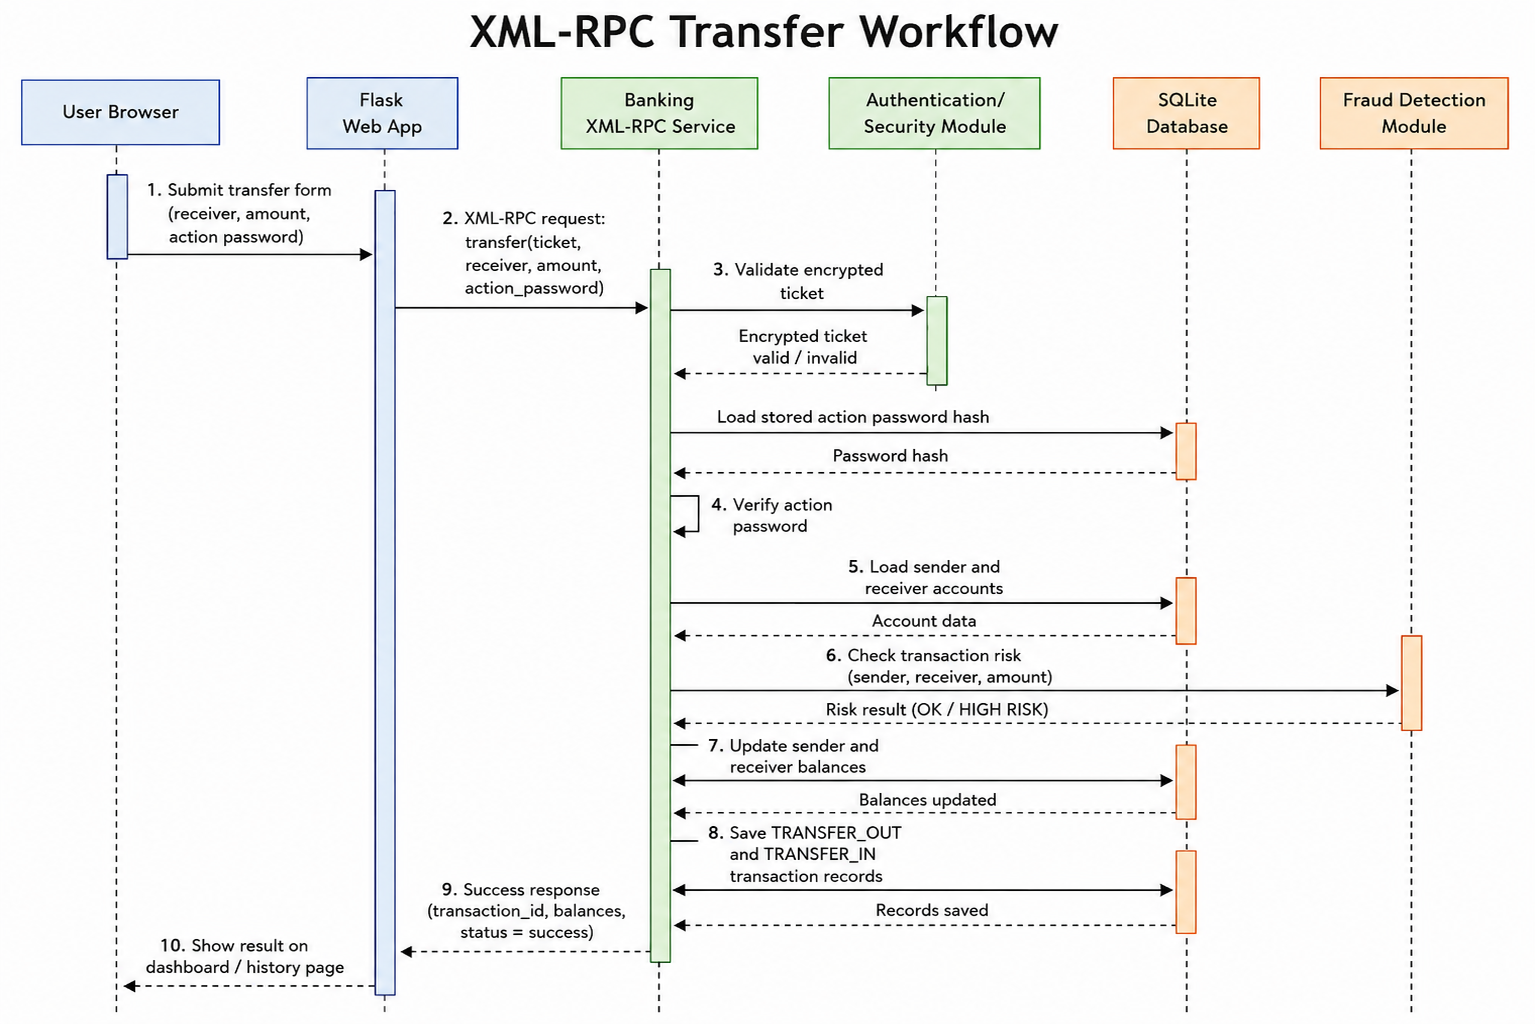
\includegraphics[width=0.92\textwidth,height=0.72\textheight,keepaspectratio]{RPC-Workflow-Diagram-GPT.png}
\end{frame}

\begin{frame}{Security Features}
    \begin{itemize}
        \item Login passwords and action passwords are stored as hashes.
        \item Login creates a time-limited Fernet encrypted ticket.
        \item Banking RPC methods validate the ticket before processing requests.
        \item Withdraw and transfer require the action password.
        \item Audit logs record important account actions.
    \end{itemize}
\end{frame}

\begin{frame}{Database Design}
    \centering
    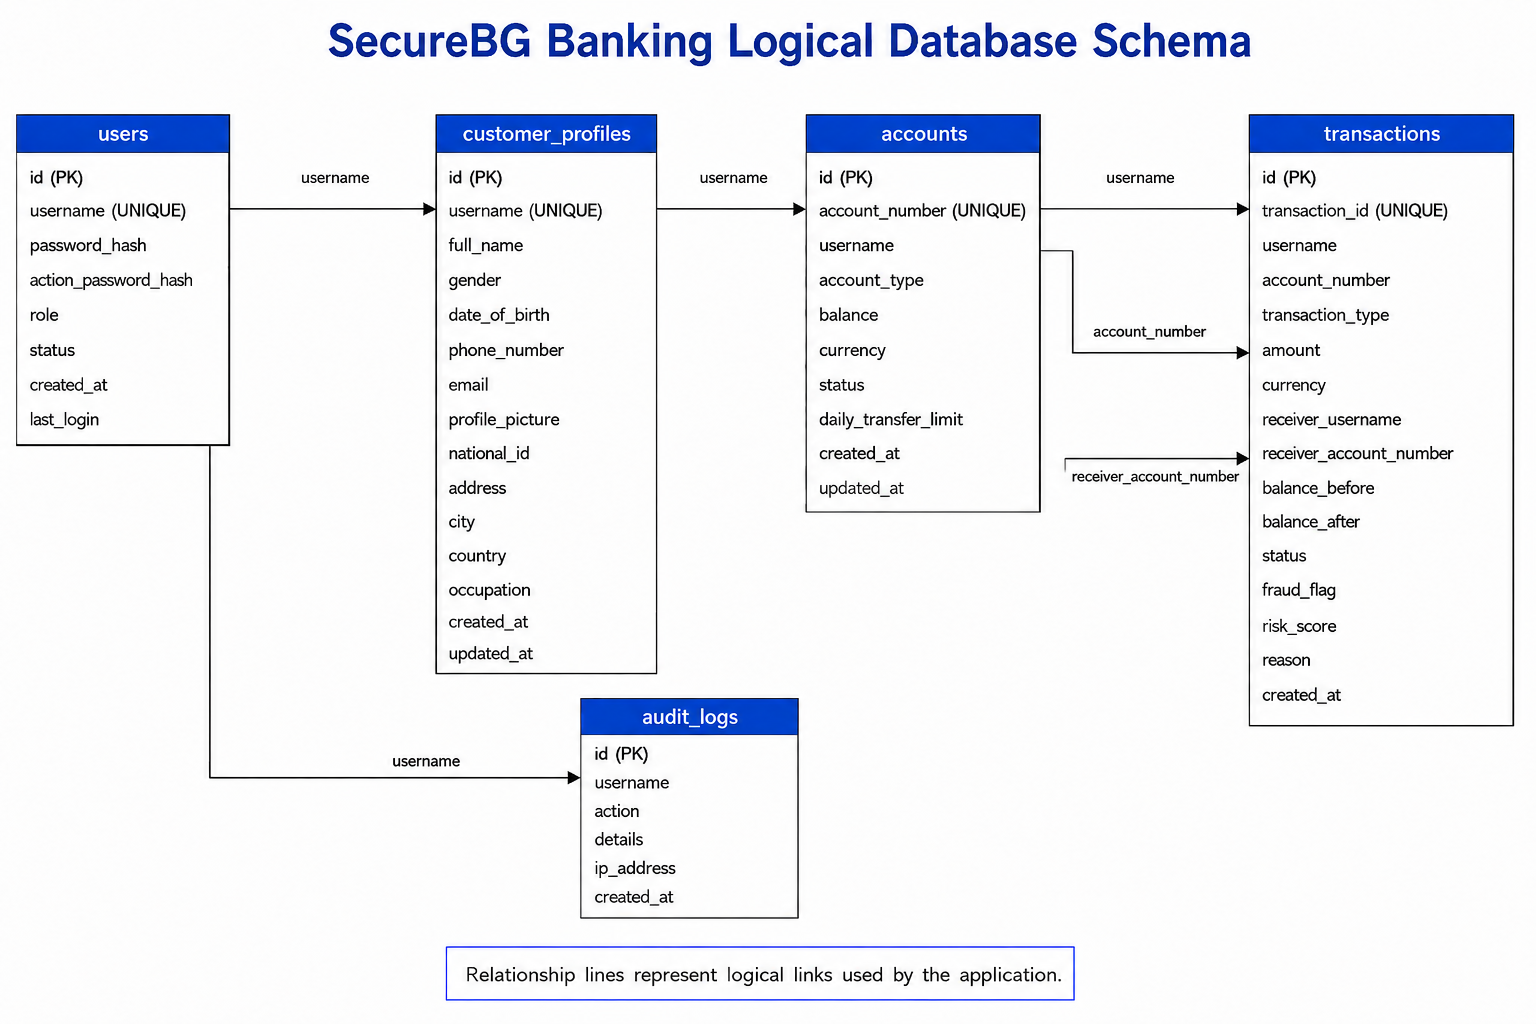
\includegraphics[width=0.92\textwidth,height=0.72\textheight,keepaspectratio]{Banking-dabase-logical-schena.png}
\end{frame}

\begin{frame}{Application Screenshots}
    \begin{columns}
        \begin{column}{0.5\textwidth}
            \centering
            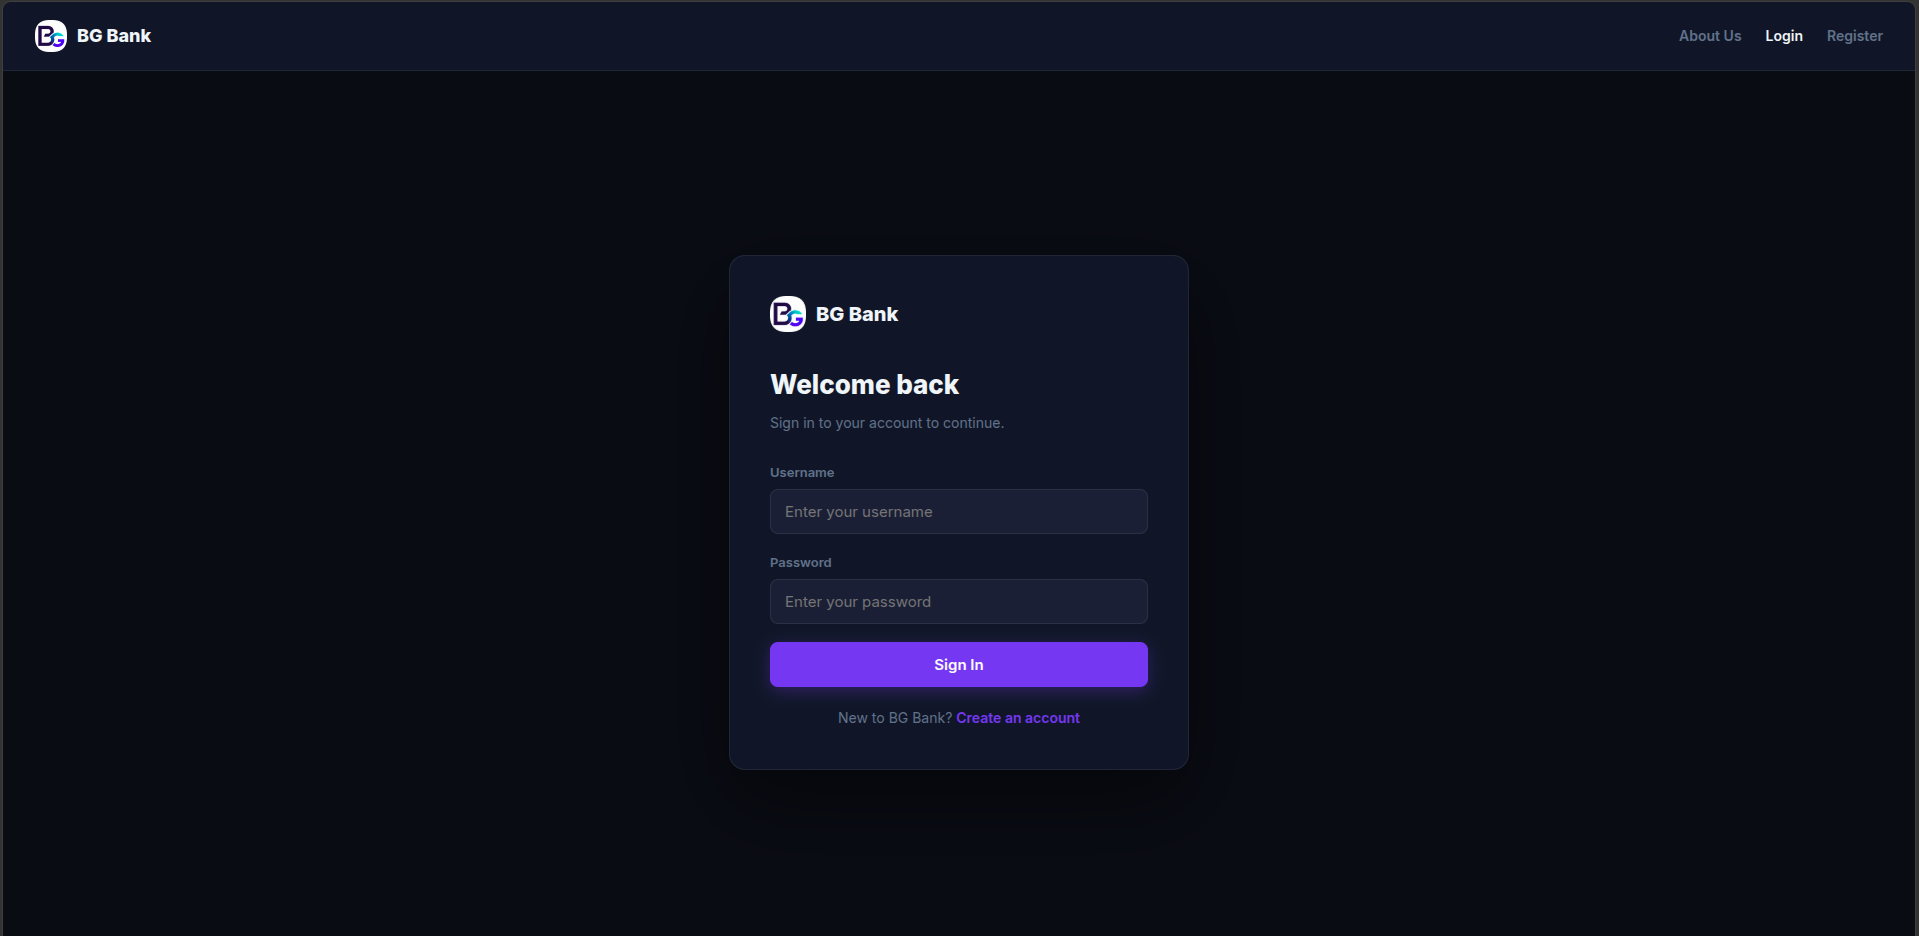
\includegraphics[width=0.95\textwidth,height=0.34\textheight,keepaspectratio]{login-web-view.png}\\[0.3cm]
            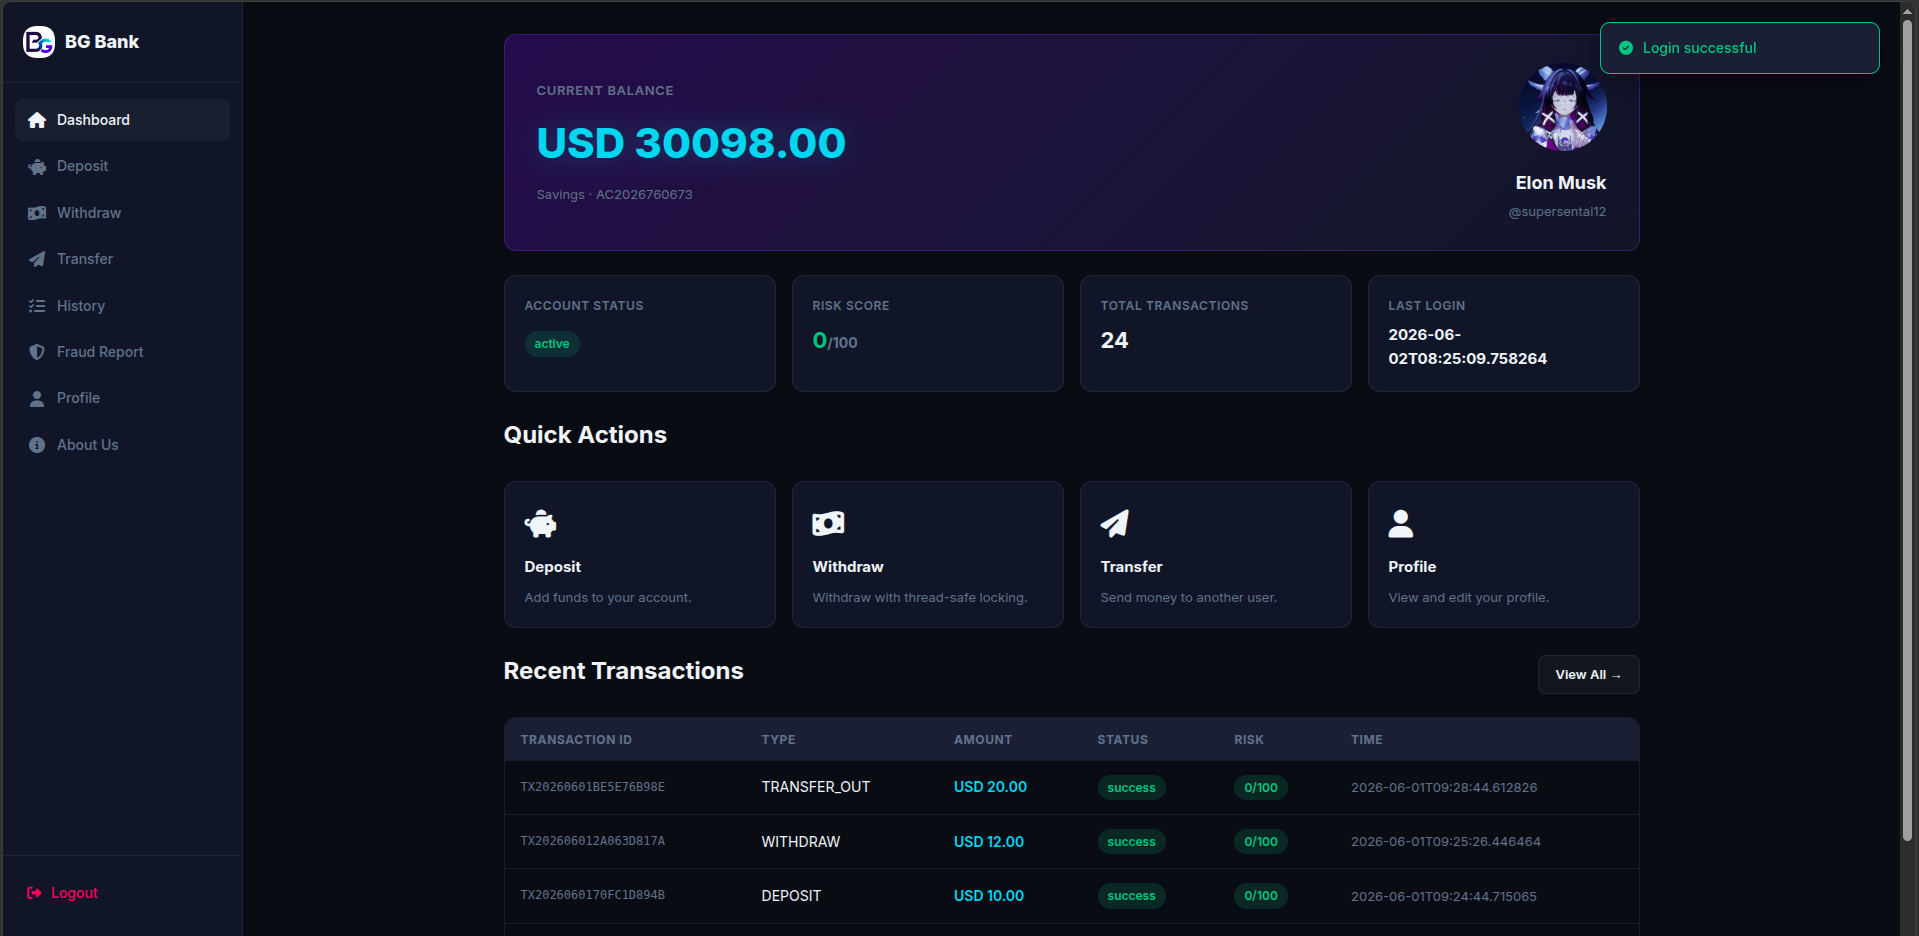
\includegraphics[width=0.95\textwidth,height=0.34\textheight,keepaspectratio]{dashboard-web-view.png}
        \end{column}
        \begin{column}{0.5\textwidth}
            \centering
            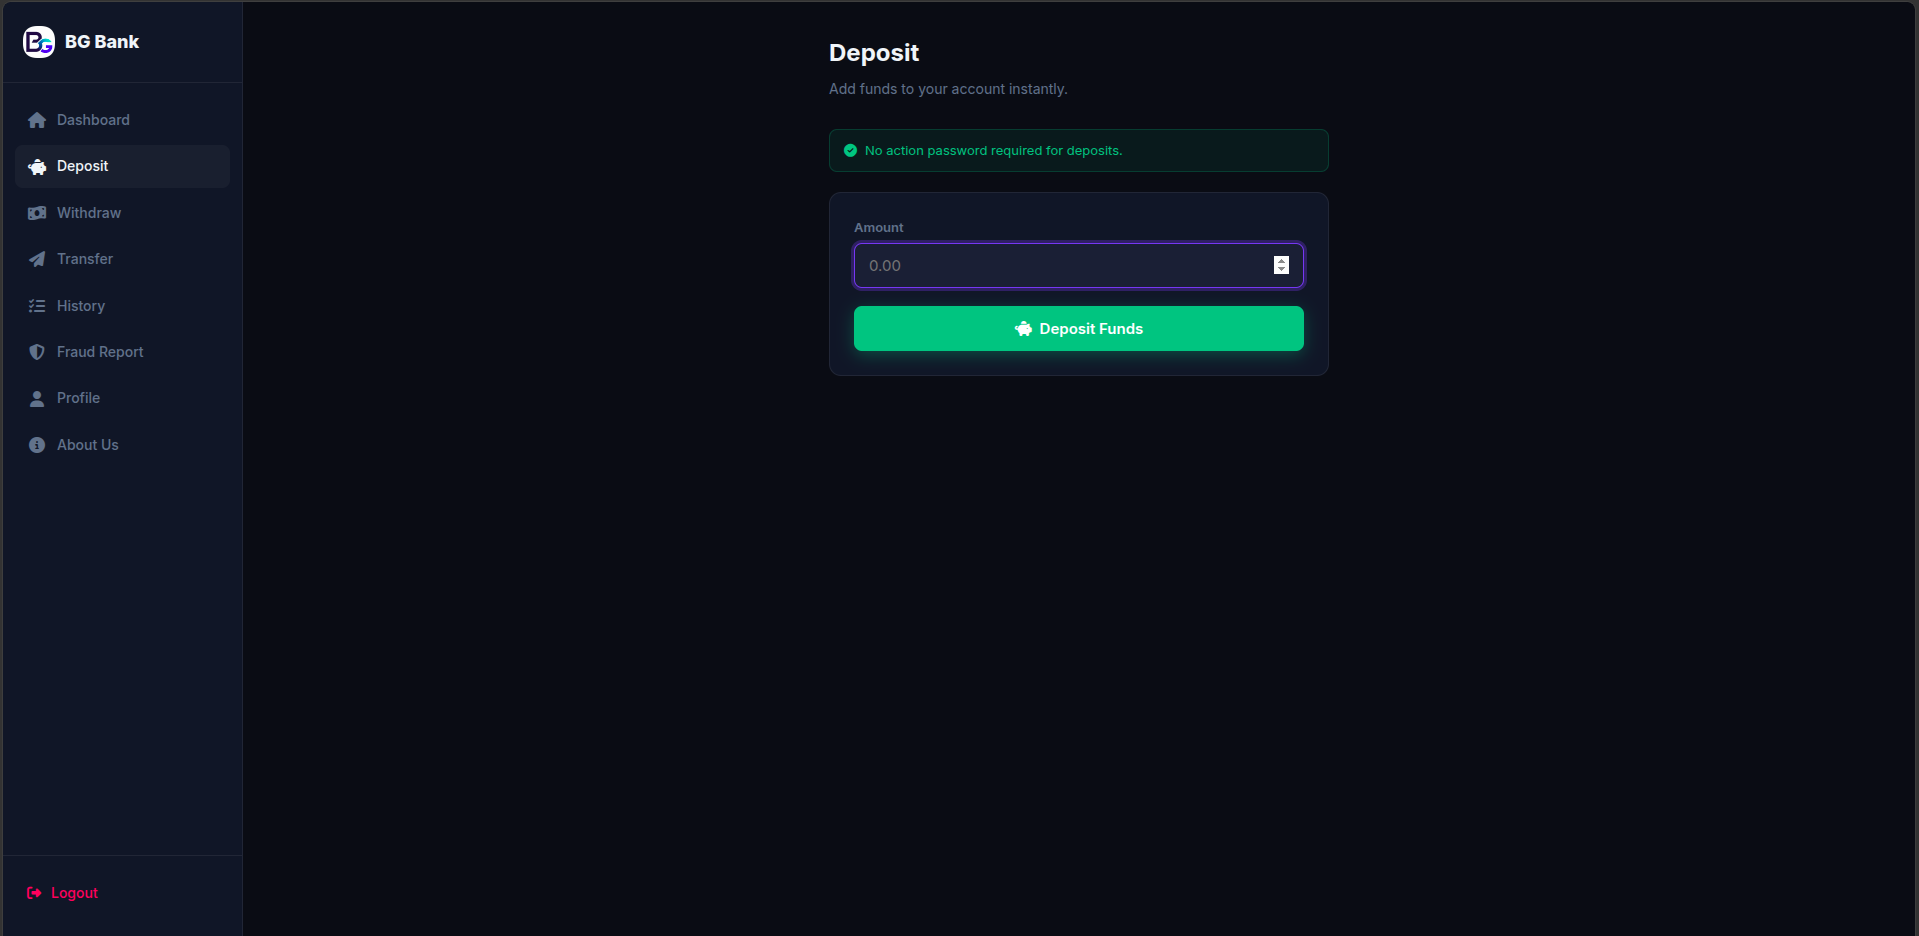
\includegraphics[width=0.95\textwidth,height=0.34\textheight,keepaspectratio]{deposit-web-view.png}\\[0.3cm]
            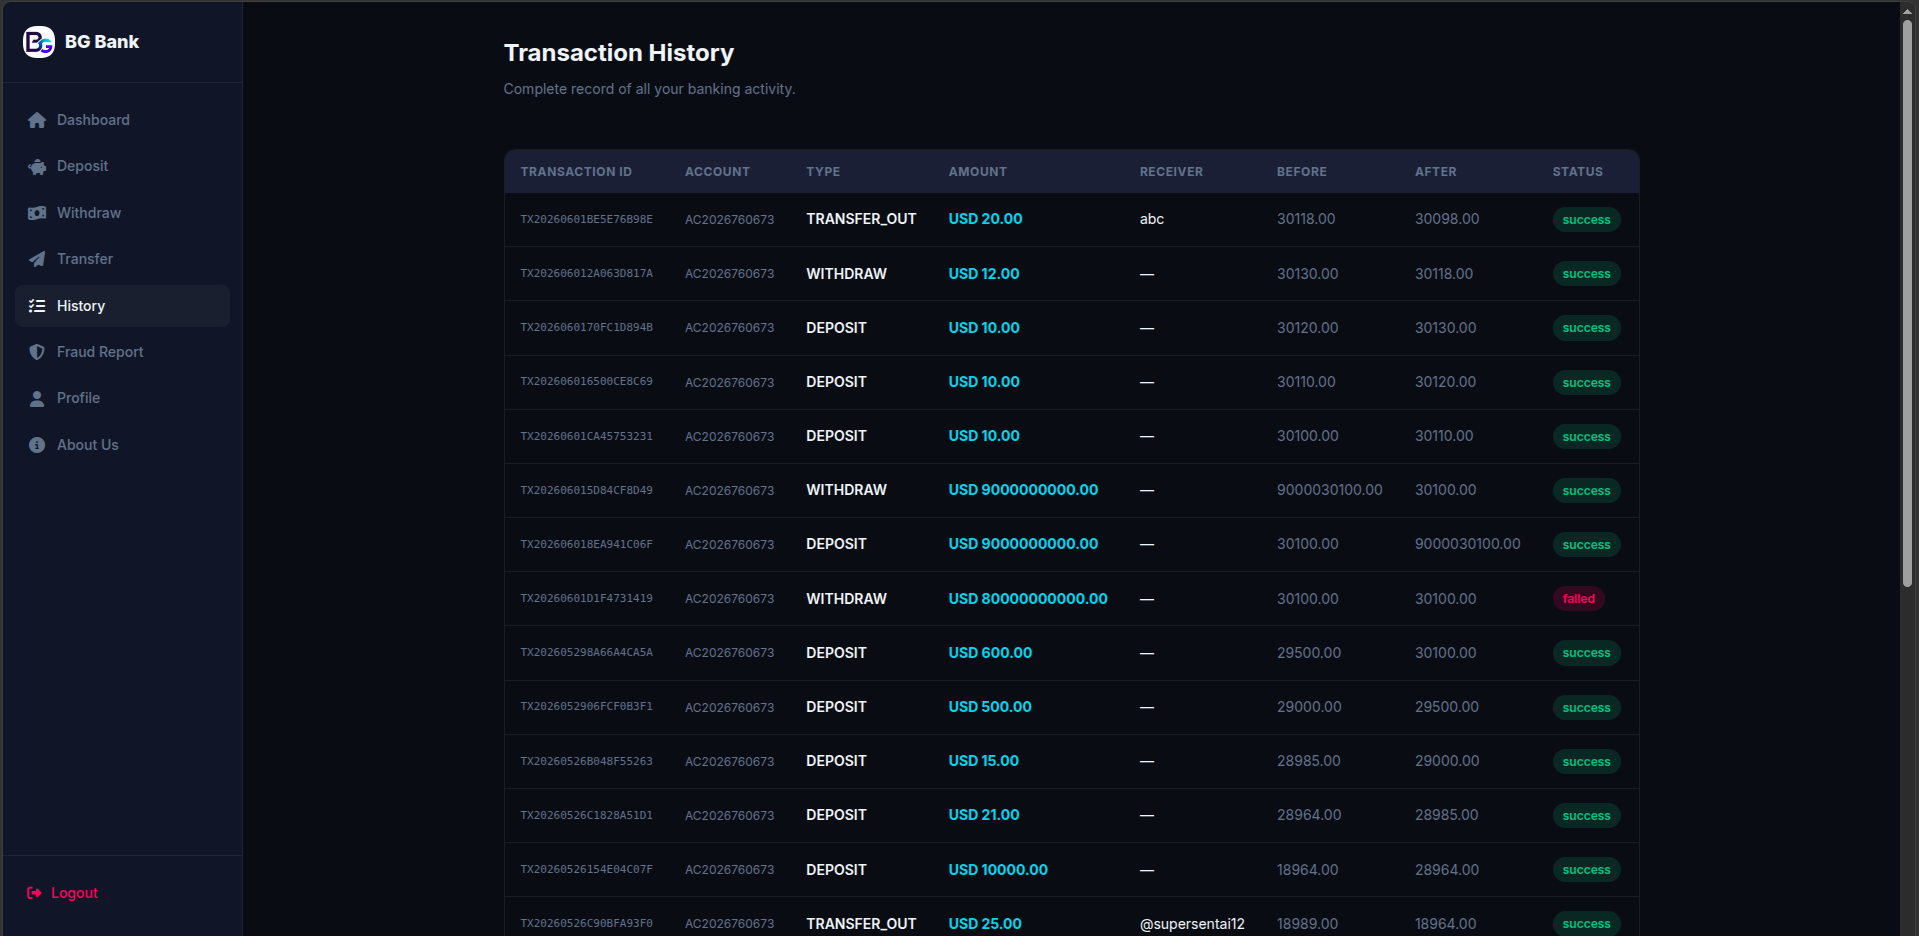
\includegraphics[width=0.95\textwidth,height=0.34\textheight,keepaspectratio]{history-web-view.png}
        \end{column}
    \end{columns}
\end{frame}

\begin{frame}{Docker Demonstration}
    \centering
    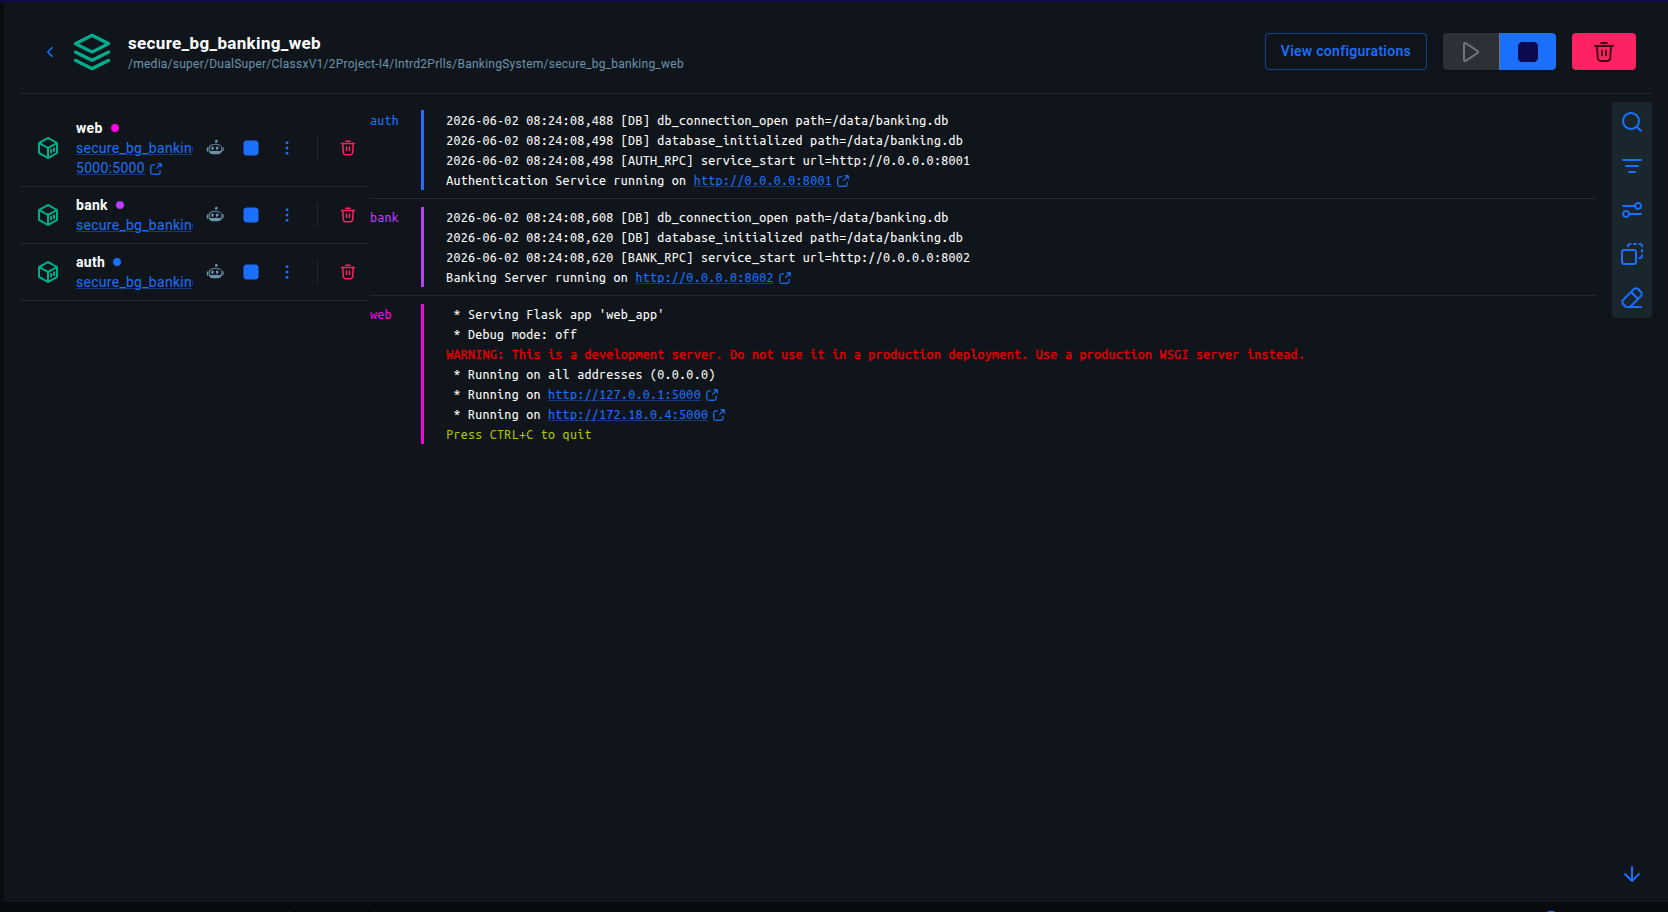
\includegraphics[width=0.92\textwidth,height=0.72\textheight,keepaspectratio]{docker-hosting-view.png}
\end{frame}

\begin{frame}{Limitations and Future Work}
    \begin{itemize}
        \item Use database transactions for registration and money operations.
        \item Store money as integer cents or Decimal values instead of floating point values.
        \item Add CSRF protection and stronger authentication controls.
        \item Add automated tests for registration, login, deposit, withdraw, and transfer.
        \item Use HTTPS and production-safe logging for deployment.
    \end{itemize}
\end{frame}

\begin{frame}{Conclusion}
    \begin{itemize}
        \item BG Bank demonstrates a distributed banking workflow using Flask and XML-RPC.
        \item The project separates authentication, banking logic, security helpers, and database storage.
        \item Encrypted tickets and action passwords improve protection for account operations.
        \item The system is suitable for demonstrating RPC communication and service coordination.
    \end{itemize}
\end{frame}

\begin{frame}
    \centering
    \Huge Thank You
\end{frame}

\end{document}
